\documentclass{tufte-handout}
\usepackage{graphicx}
\usepackage{changepage}
\usepackage{amsmath}
\usepackage{float}

\definecolor{SolutionColor}{rgb}{0.5,0,0}
\newcommand{\solution}[1]{
\begin{adjustwidth}{1cm}{}
\textit{\color{SolutionColor} #1}
\end{adjustwidth}}
\usepackage{lipsum}
\newcommand\tab[1][1cm]{\hspace*{#1}}

\begin{document}

\begin{fullwidth} 
\section{MATH1010: Homework 1}
    \textit{Assigned January 17, 2022}
    \textbf{Due January 24, 2022}
    \vspace{.2cm}
    
\noindent\textit{Exercises taken from Easley and Kleinberg are reproduced here and referenced as \textbf{E\&K, Chapter X, Problem Y.}}    

\section*{\textbf{Exercise 1}}
\textit{Homophily}\\
Use the graph in Figure 1 to answer the following questions:
\begin{figure*}[!h]
    \centering
    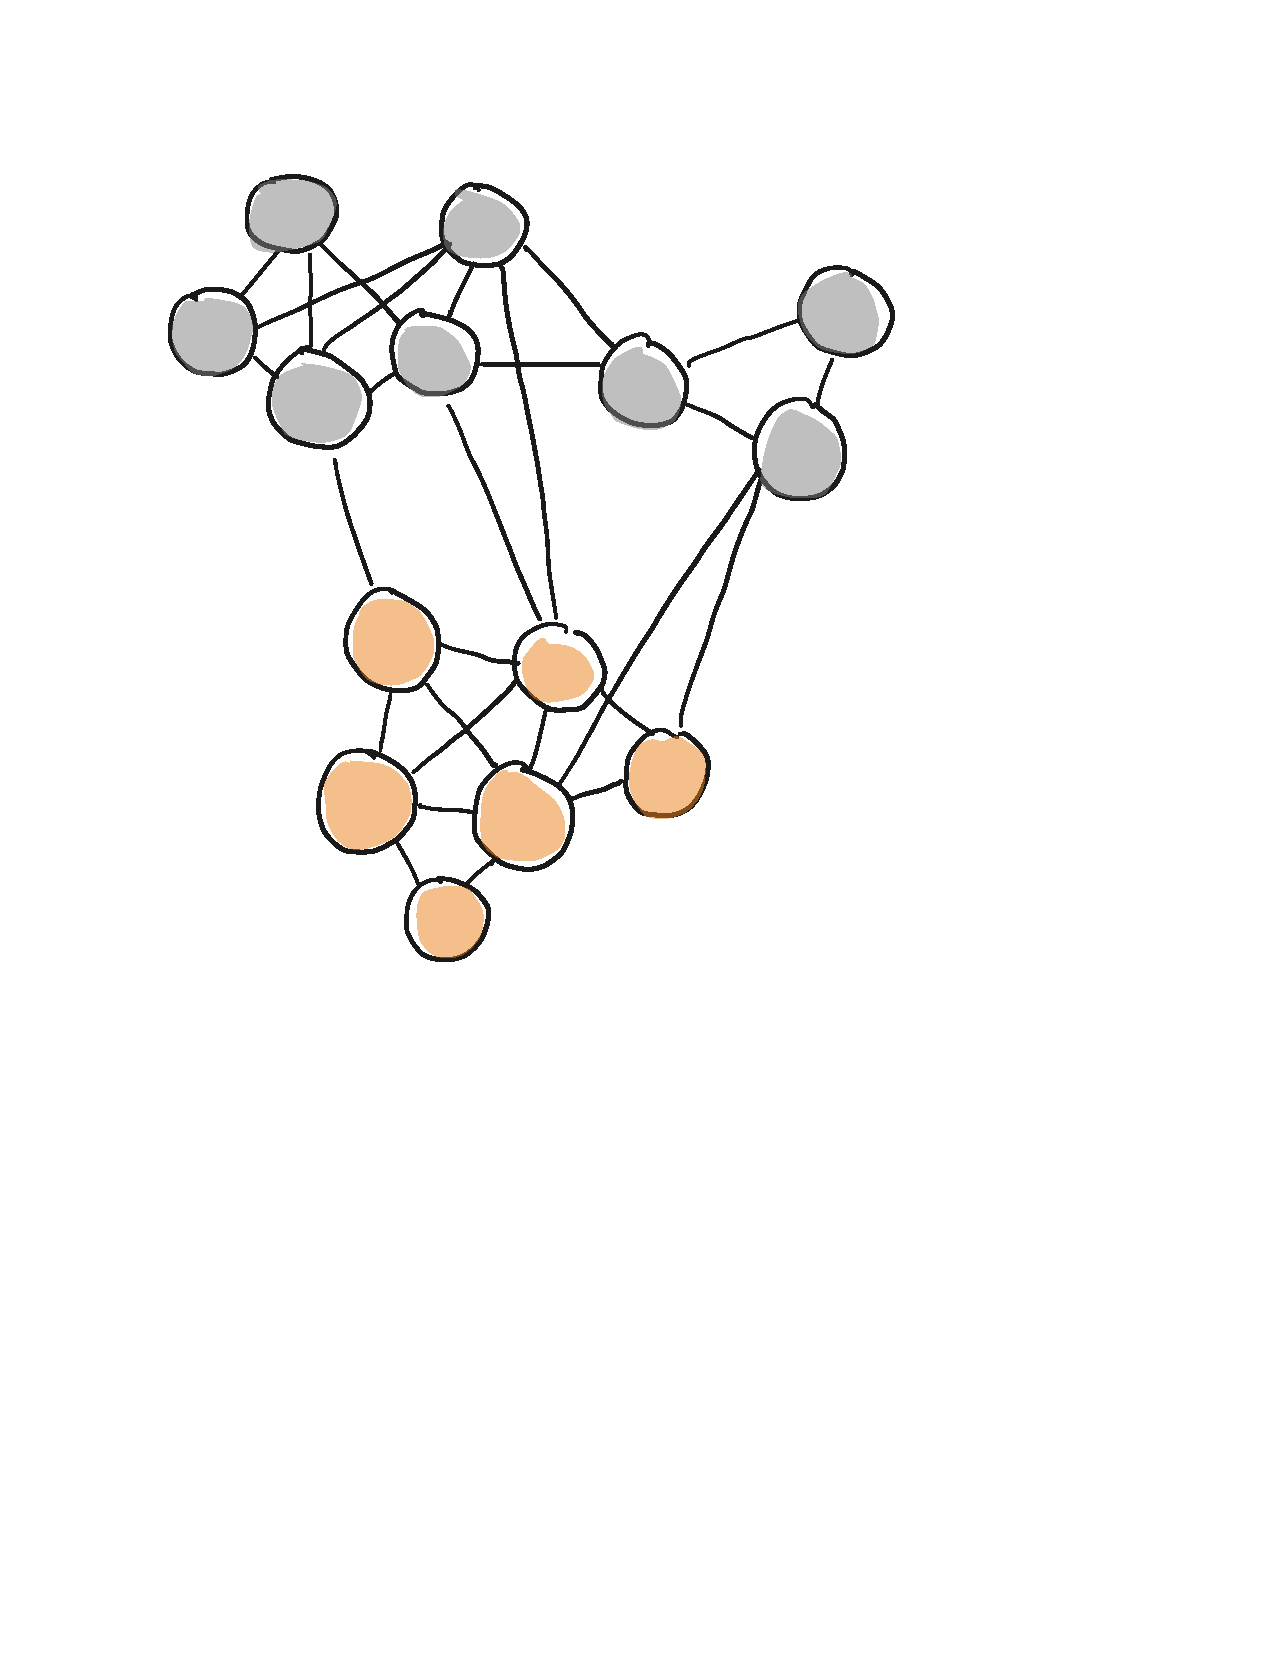
\includegraphics[width = .3\textwidth]{homophily.pdf}
    \caption{The graph for Exercise 1}
\end{figure*}
\begin{enumerate}
    \item What percent of the 28 edges in this graph are heterogeneous?
    \item What percent of the edges do we \textit{expect} to be heterogeneous if nodes are randomly typed? \textit{Hint, see section 4.1 of the textbook.}
    \item Based on 1. and 2., is there evidence for homophily in this graph?
\end{enumerate}
% \solution{
% You can type your answer here
% }
\section*{\textbf{Exercise 2}}
\textit{Homophily, part II}\\
Use the graph in Figure 2 to answer the following questions:
\begin{figure*}[!h]
    \centering
    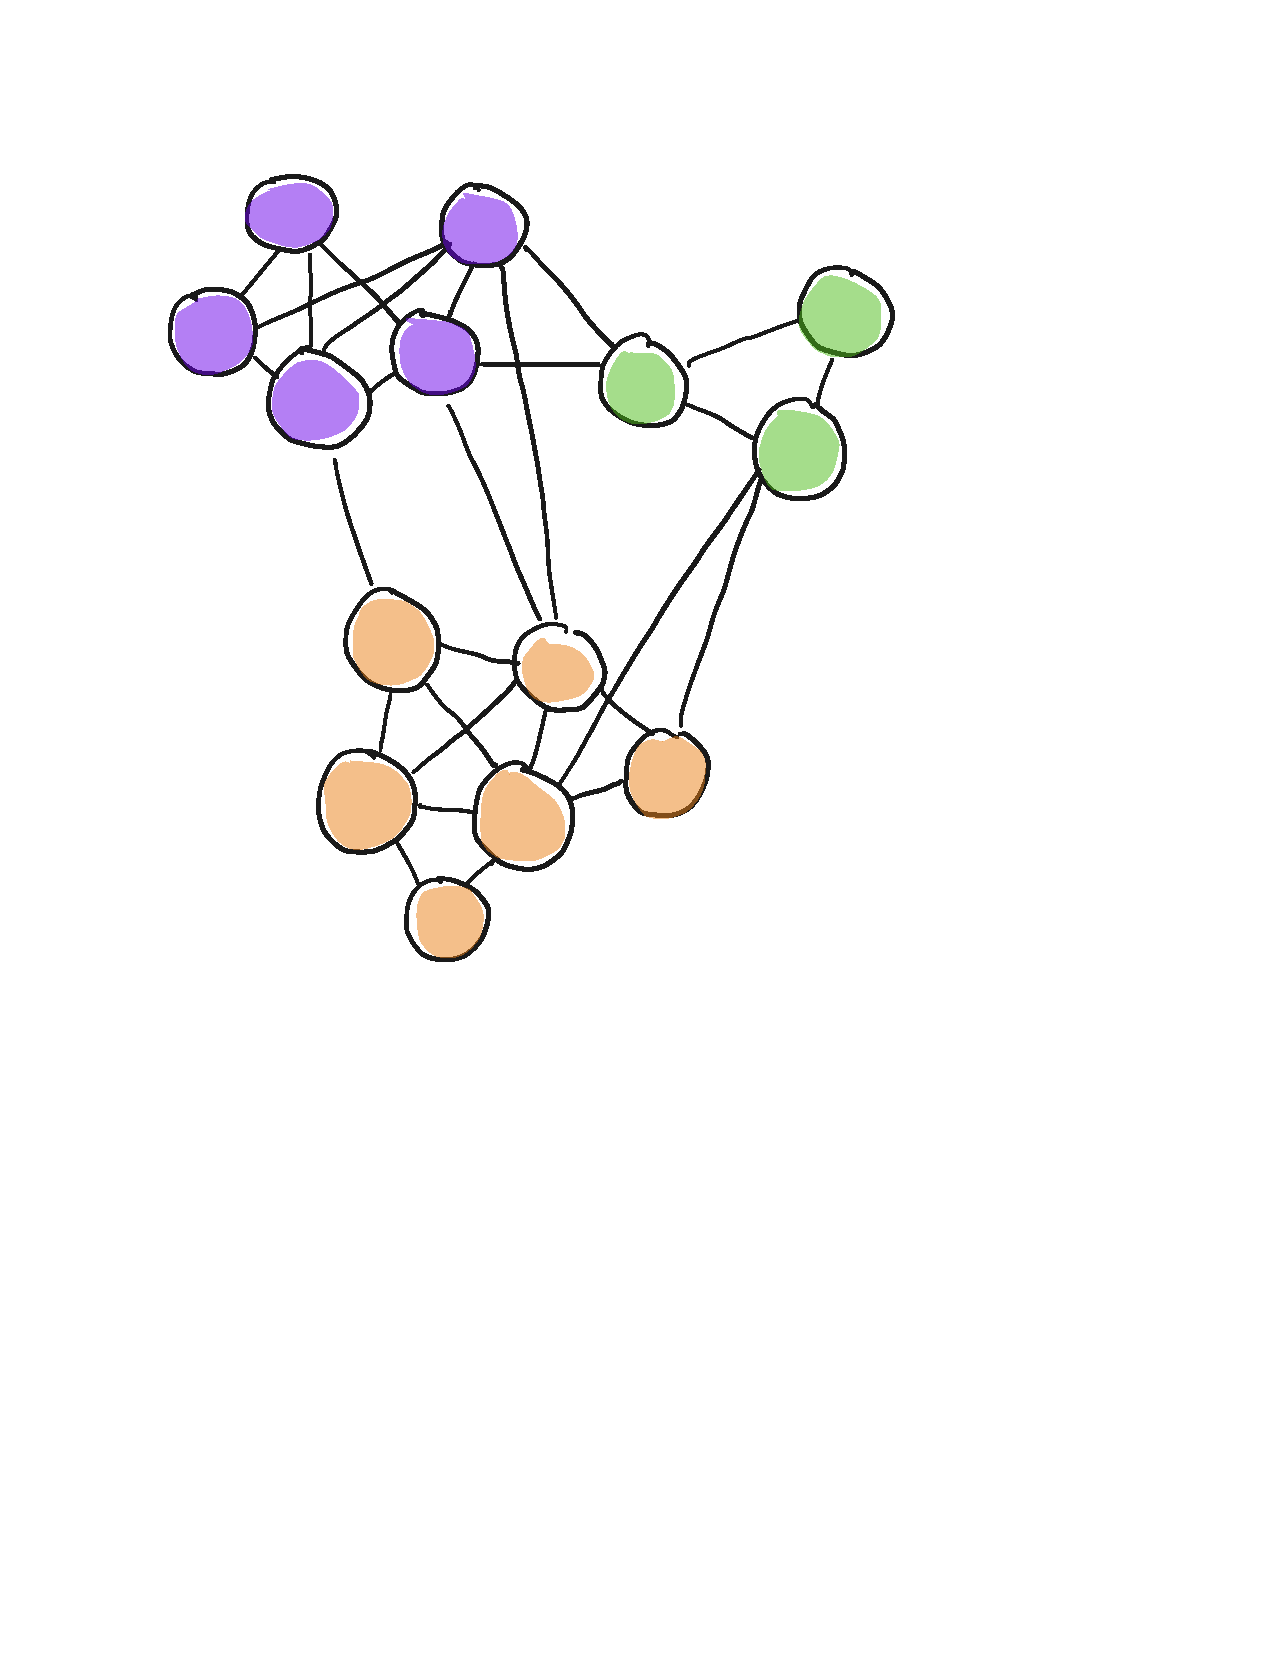
\includegraphics[width = .25\textwidth]{homophilyII.pdf}
    \caption{The graph for Exercise 2}
\end{figure*}
\begin{enumerate}
    \item What percent of the 28 edges in this graph are between a purple and orange node?
    \item What percent of the edges in this graph are between a purple and green node?
    \item What percent of the edges in this graph are between an orange and green node?
    \item Using the same reasoning as described in section 4.1 of the textbook, what percent of the edges do we \textit{expect} to be between a purple and orange node if nodes are randomly typed?
    \item What percent of the edges do we \textit{expect} to be between a purple and green node if nodes are randomly typed?
    \item What percent of the edges do we \textit{expect} to be between a green and orange node if nodes are randomly typed?
    \item Interpret your above answers in the context of what we've learned about homophily.
\end{enumerate}
\section*{\textbf{Exercise 3}}
\textit{Mechanisms underlying homophily}\\
The graphs in Figure 3 represent snapshots of the same network over 4 different weeks. Their order is shown chronologically.
\begin{figure*}[!h]
    \centering
    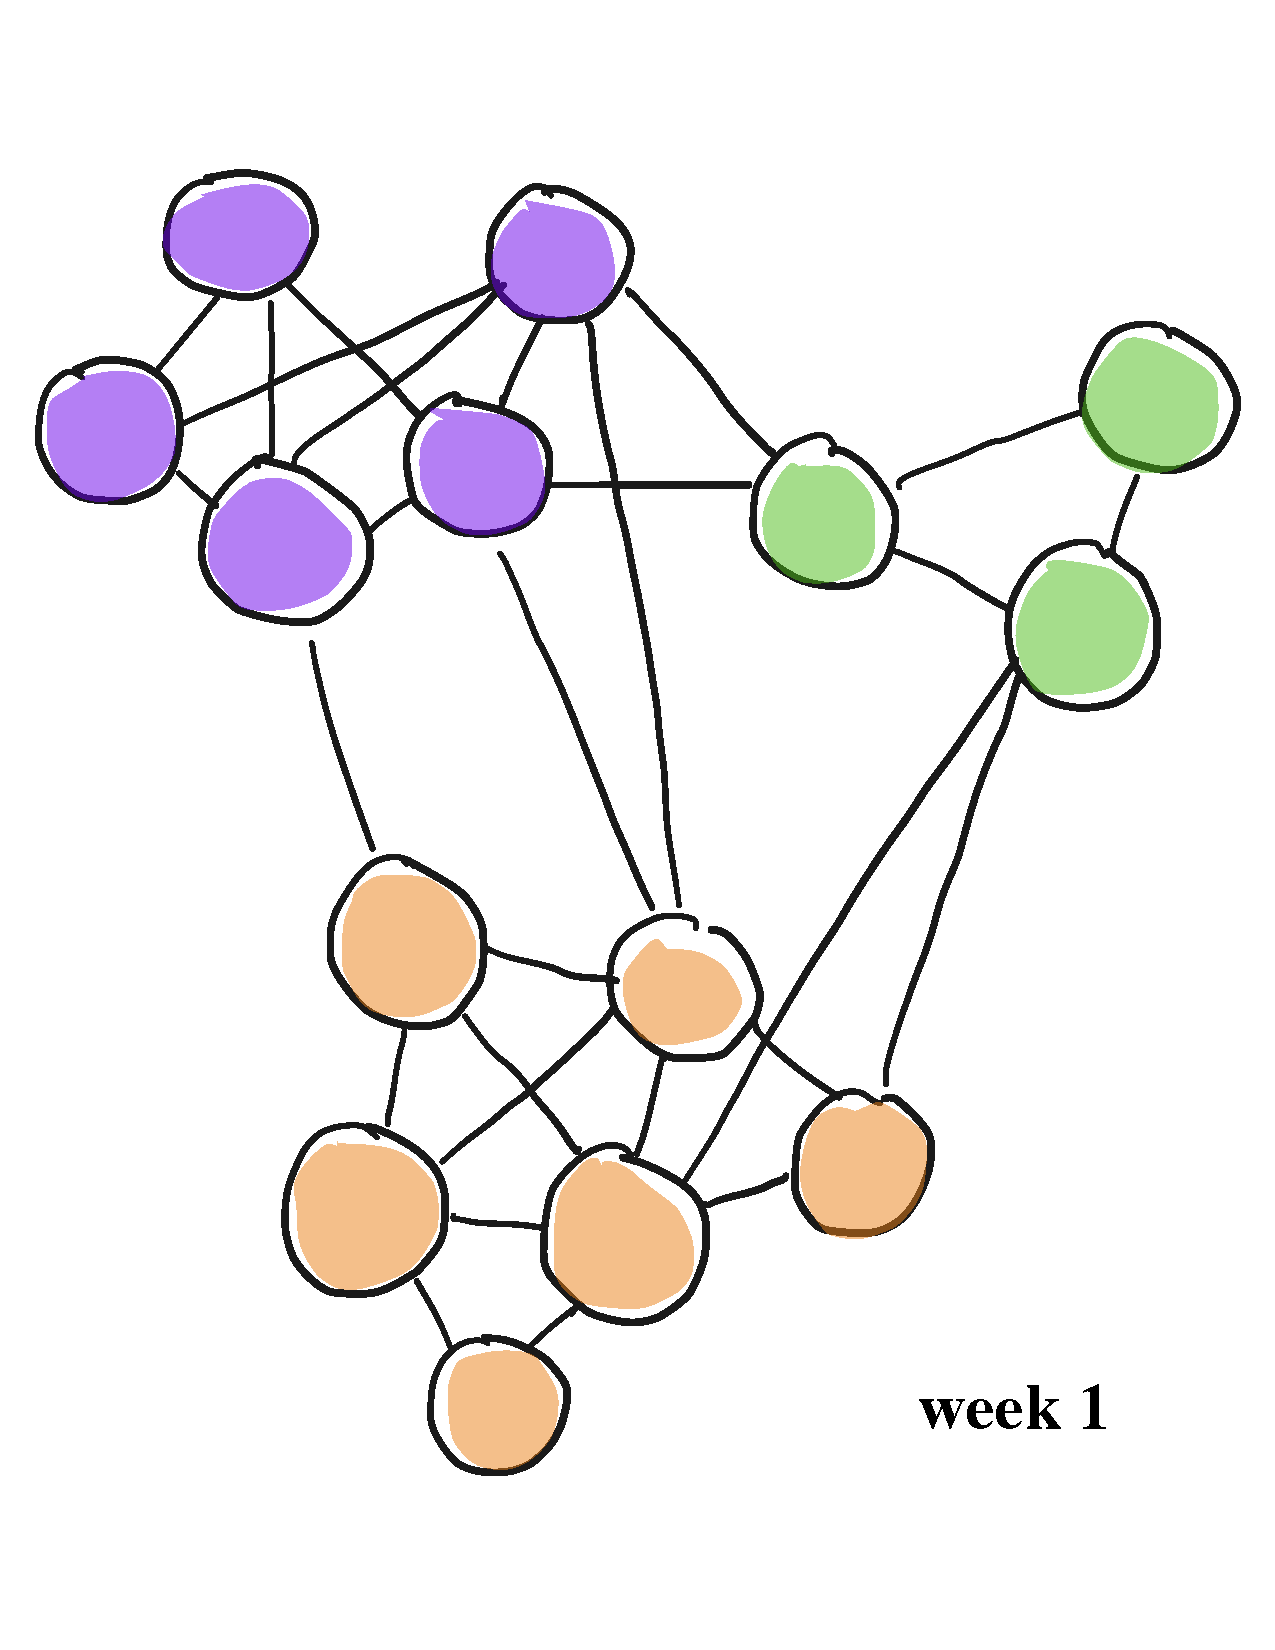
\includegraphics[width = .25\textwidth]{timei.pdf}
    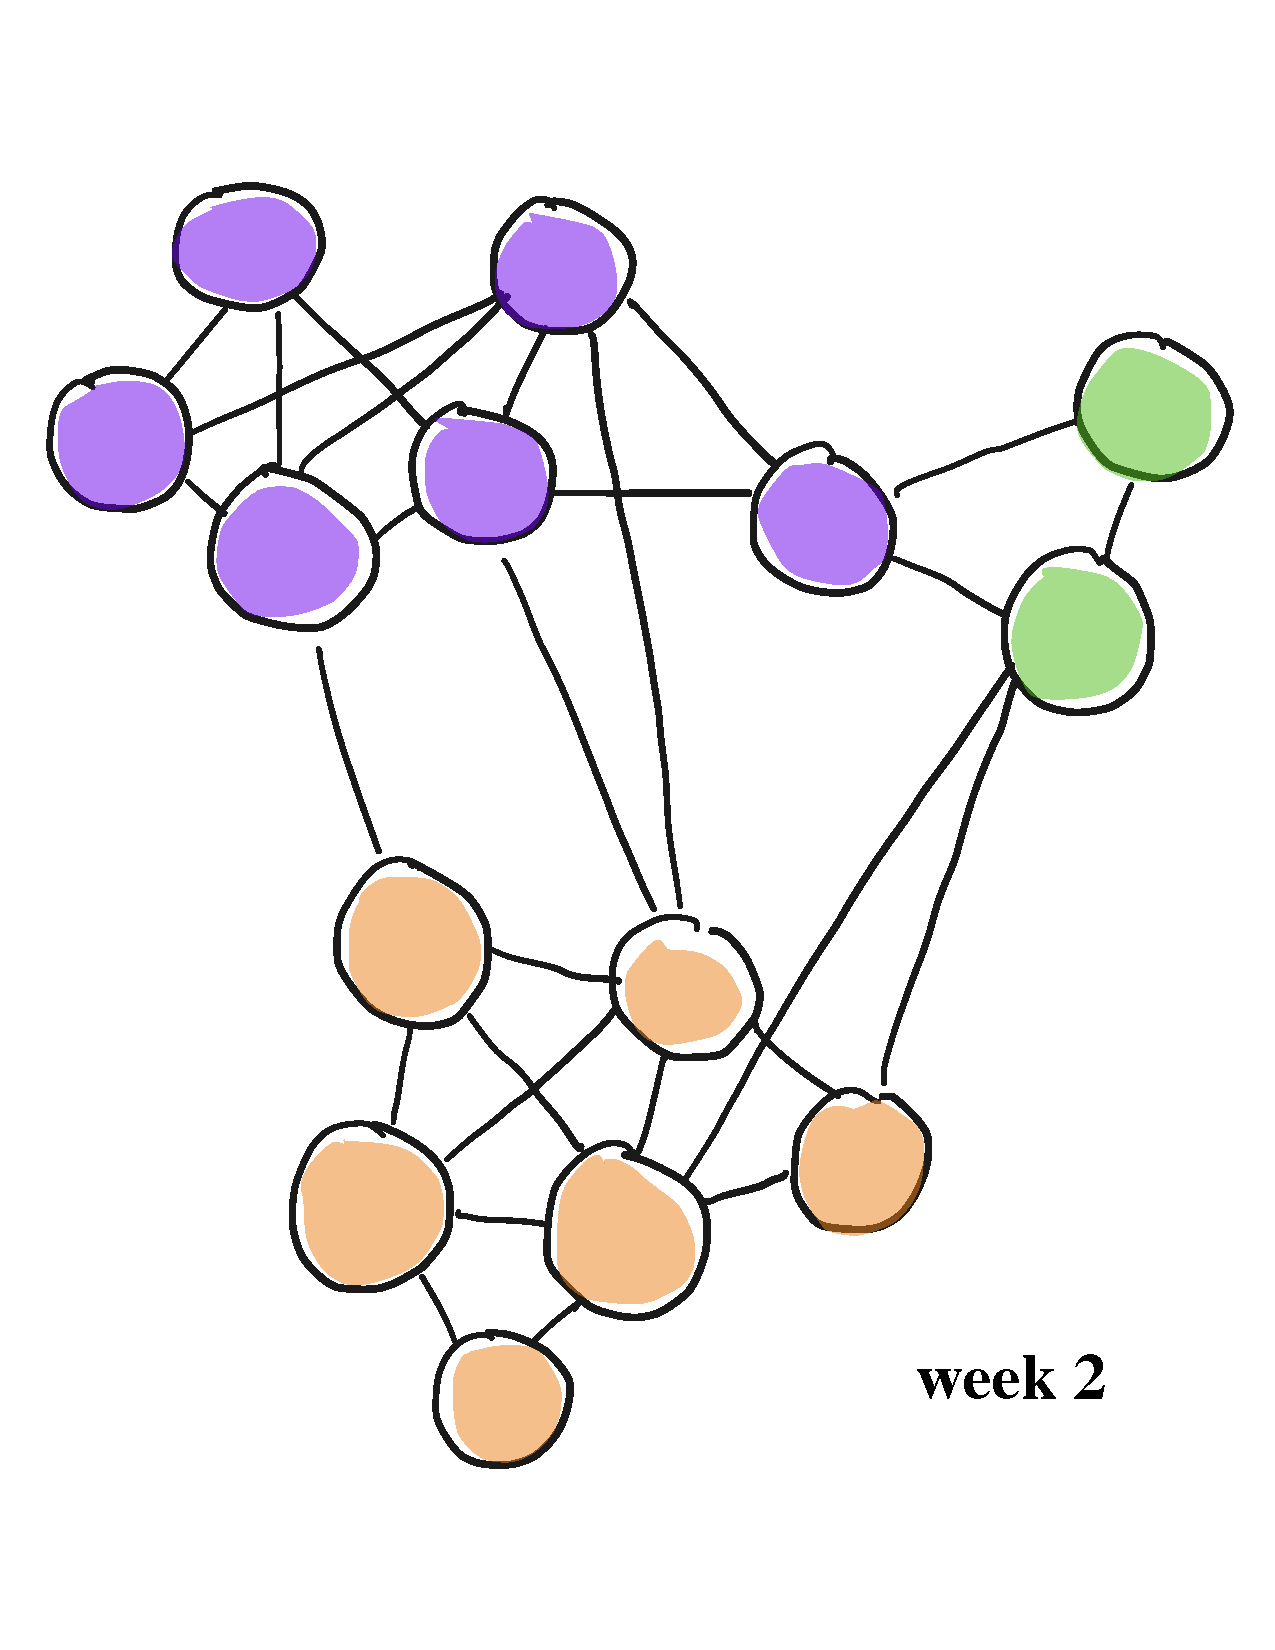
\includegraphics[width = .25\textwidth]{timeii.pdf}\\
    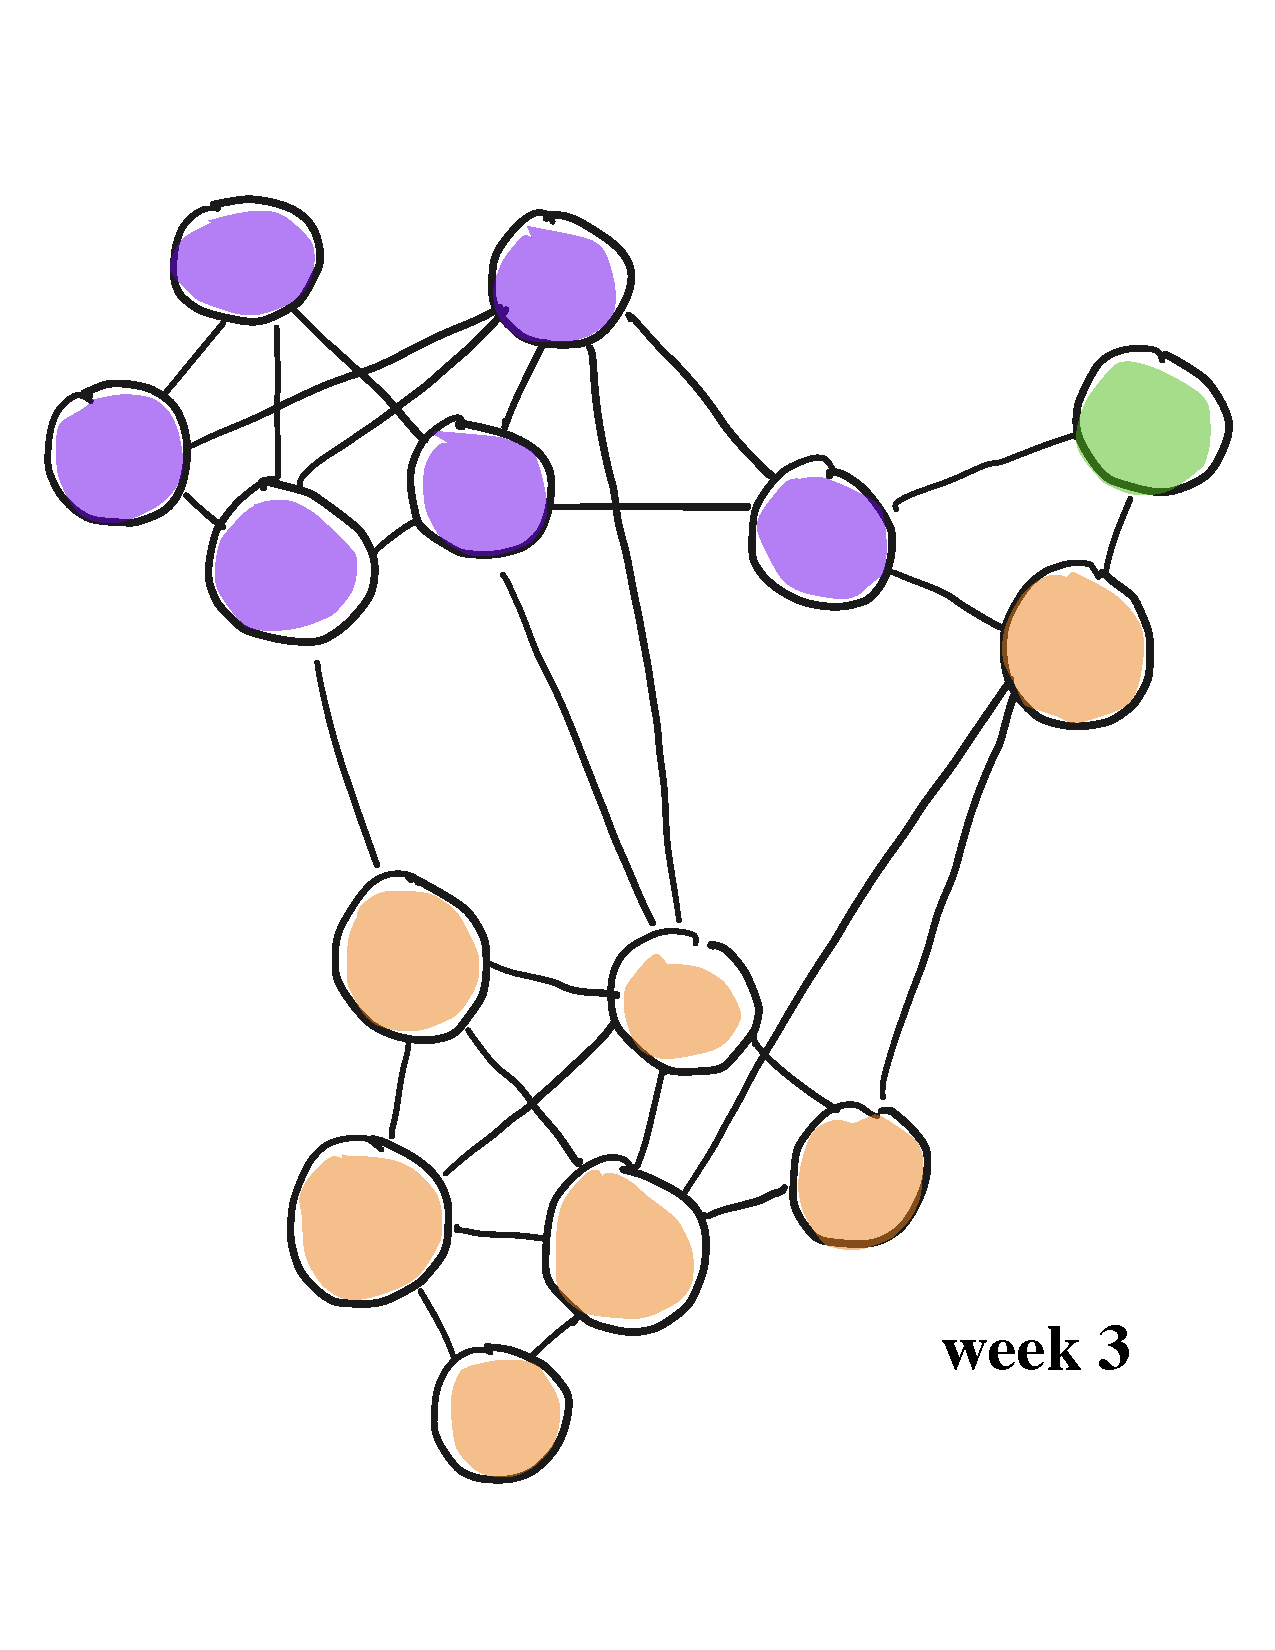
\includegraphics[width = .25\textwidth]{timeiii.pdf}
    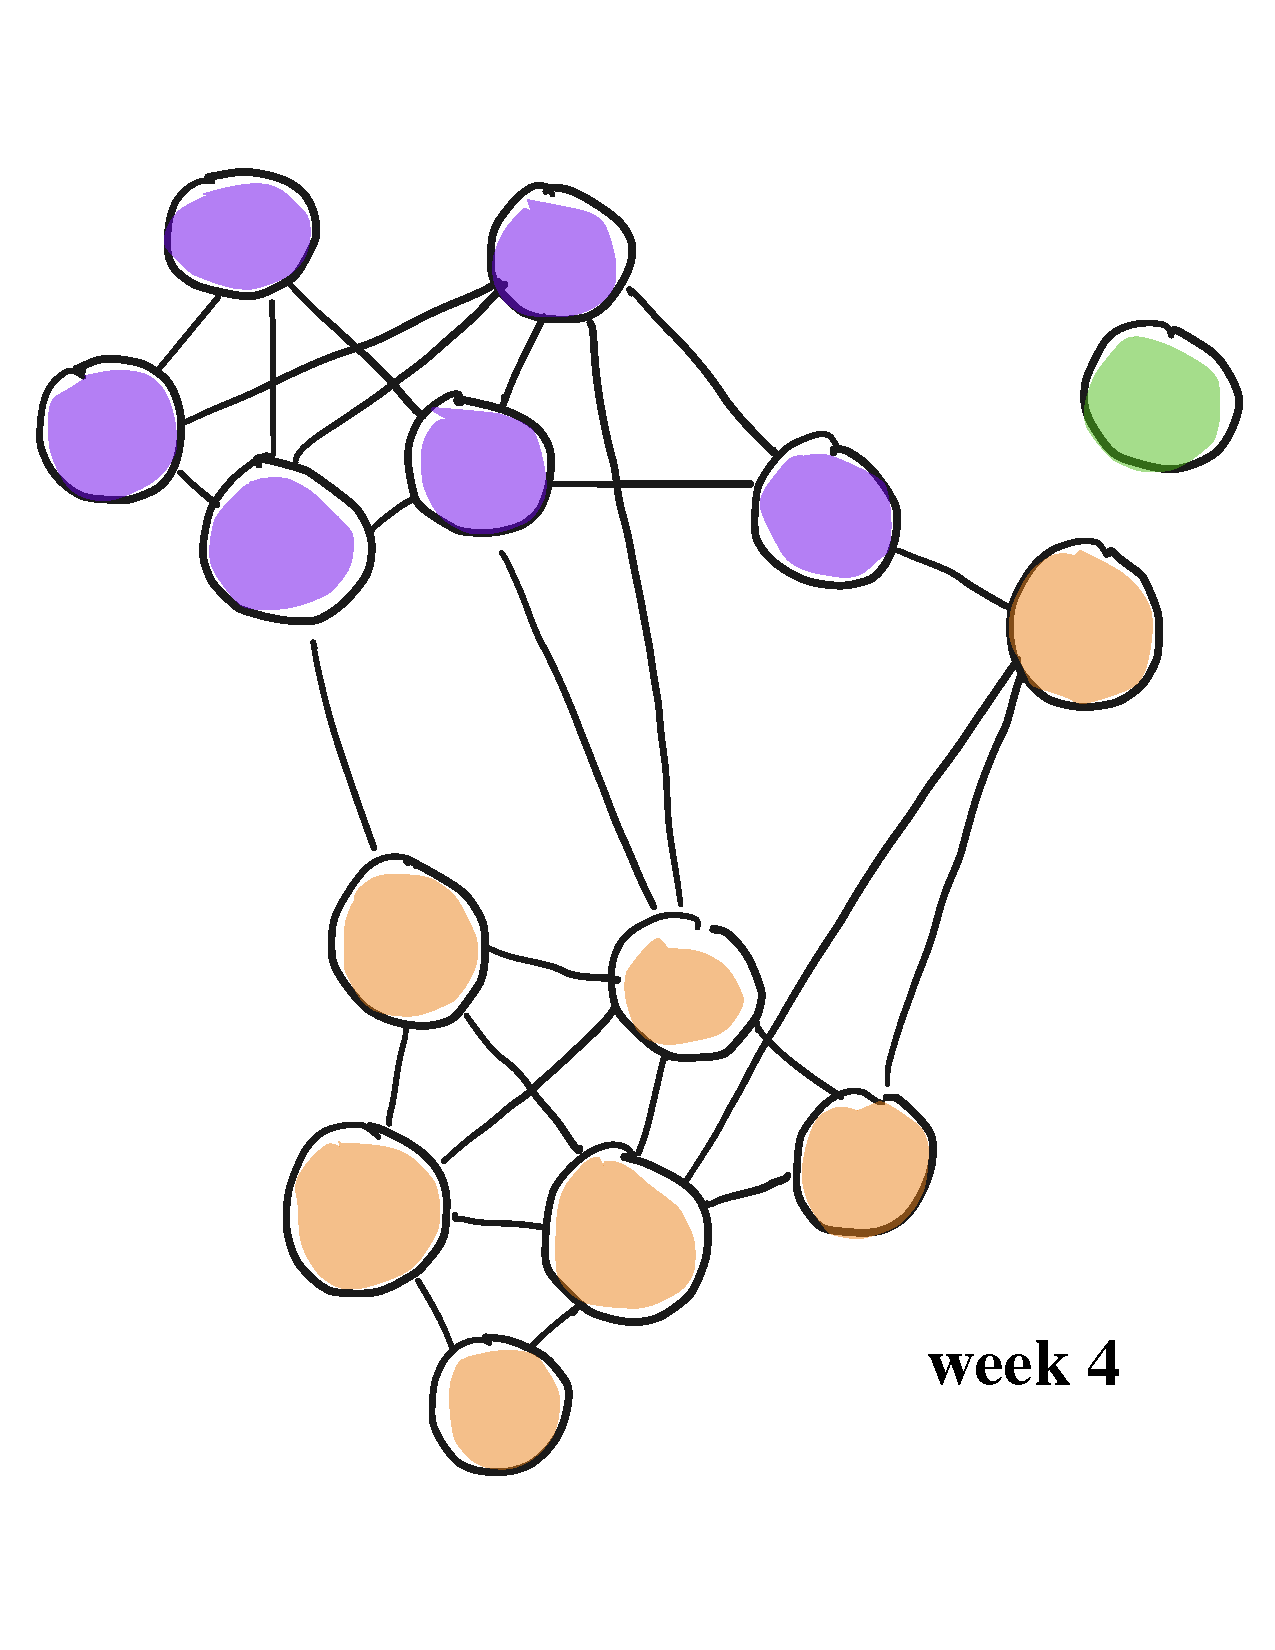
\includegraphics[width = .25\textwidth]{timeiv.pdf}
    \caption{The same network, captured over four different weeks.}
\end{figure*}
\vspace{.2cm}\\
What mechanisms underlying homophily can you attribute each change in the graph to? Why do you think so?
\section*{\textbf{Exercise 4}}
\textit{E\&K, Chapter 4, Problem 2.}\\
Given a bipartite affiliation graph, showing the membership of people in different social foci, researchers sometimes create a \textit{projected graph} on just the people, in which we join two people when they have a focus in common.
\begin{enumerate}
    \item Draw what such a projected graph would look like for the example of memberships on corporate boards of directors from Figure 4.4. Here the nodes would be the seven people in the figure, and there would be an edge joining any two who serve on a board of directors together.
    \item Give an example of two different affiliation networks — on the same set of people, but with different foci-- so that the projected graphs from these two different affliation networks are the same. This shows how information can be ``lost'' when moving from the full affiliation network to just the projected graph on the set of people.
\end{enumerate}
\begin{figure*}[!h]
    \centering
    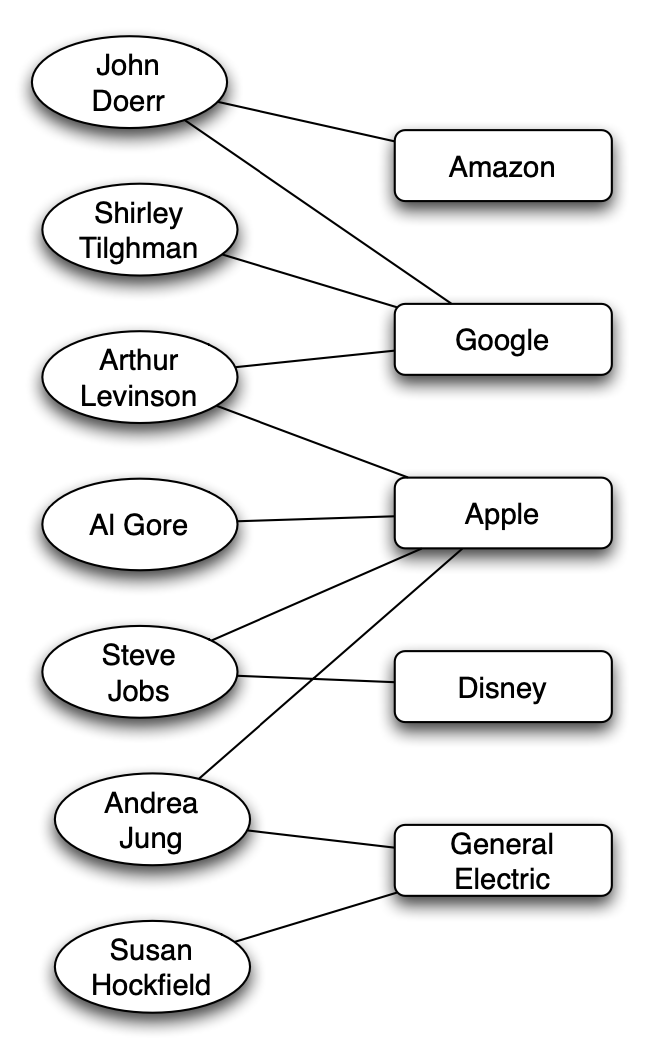
\includegraphics[width = .27\textwidth]{ek444.png}
    \caption{Figure 4.4 from E\&K, for exercise 3}
\end{figure*}

\end{fullwidth}
\end{document}
